% !TeX spellcheck = en_US
\documentclass[12pt,a4paper,twocolumn]{article}
\usepackage[utf8]{inputenc}
\usepackage[T1]{fontenc}
\usepackage{amsmath}
\usepackage{amssymb}
\usepackage{graphicx}
\usepackage{fancyhdr}
\usepackage[english]{babel}
\usepackage{geometry}
\usepackage[dvipsnames]{xcolor}
\usepackage[english]{babel}
\usepackage{hyperref}
\usepackage[style=numeric, url=true, doi=true, isbn=false]{biblatex}

\title{Clustering with a Convolutional Variational Autoencoders of Photoplethysmography Timeseries}
\author{Lorenzo Barsotti}

\addbibresource{bibliografia.bib}
%\bibliographystyle{plain}
\geometry{ margin=2cm}
\pagestyle{fancy}
\begin{document} \thispagestyle{empty}
	%\maketitle
	
	\twocolumn[{%
		\begin{@twocolumnfalse}
		\huge \bfseries Clustering with a Convolutional Variational Autoencoders of Photoplethysmography Time-Series
		\begin{flushright}
			\large \bfseries Author: Lorenzo Barsotti	
		\end{flushright}
		
			\begin{abstract}
				The purpose of this project is to analyze photoplethysmography data, with a Convolutional Variational Auto-encoder Neural Network. In particular we would like to see if there are some \emph{latent characteristics} that allow us to discriminate the biological age of a patient from its photoplethysmogram.
				
			\end{abstract}
		\end{@twocolumnfalse}
	}]

	\section{Introduction}
		The purpose of this project is to try to estimate the biological age of a patient, from its photoplethysmogram. A photoplethysmogram is the optically obtained signal related to the changes of volume in the blood vessels (section \ref{ppg_intro}). In order to perform the age estimation I used a database composed of about 4770 photoplethysmograms of as many patients, and a \emph{Convolutional Variational Auto-Encoder}. This is a particular case of \emph{Deep Neural Network} as it will be described in the section \ref{vae_intro}. To develop the Neural Network Tensorflow 2.9.0 \cite{tensorflow2015-whitepaper} was used.
	\subsection{Photoplethysmography}
		\label{ppg_intro}
		\emph{Photoplethysmography} is a technique that use light in order to detect changes in volumes in blood vascular vessels. A \emph{Light Emitting Diode} (LED), illuminates a high vascularized body part covered by a thin layer of skin, usually a fingertip, and a photodiode measures the amount of light transmitted or reflected. In the particular case of this project, the data were taken with camera module of smartphones: the LED illuminates a fingertip and the camera records the backscattered light. 
		A \emph{photoplethysmogram} (PPG)is the plot of the recorded data of the photodiode. It is a graph in which we are able to see how  of the blood vessels' volume change over time. Ideally the obtained time series is very regular and the present peaks corresponds to patient's  heartbeat (Figure \ref{fig:ppgexample}).
		\begin{figure}[h!]
			\centering
			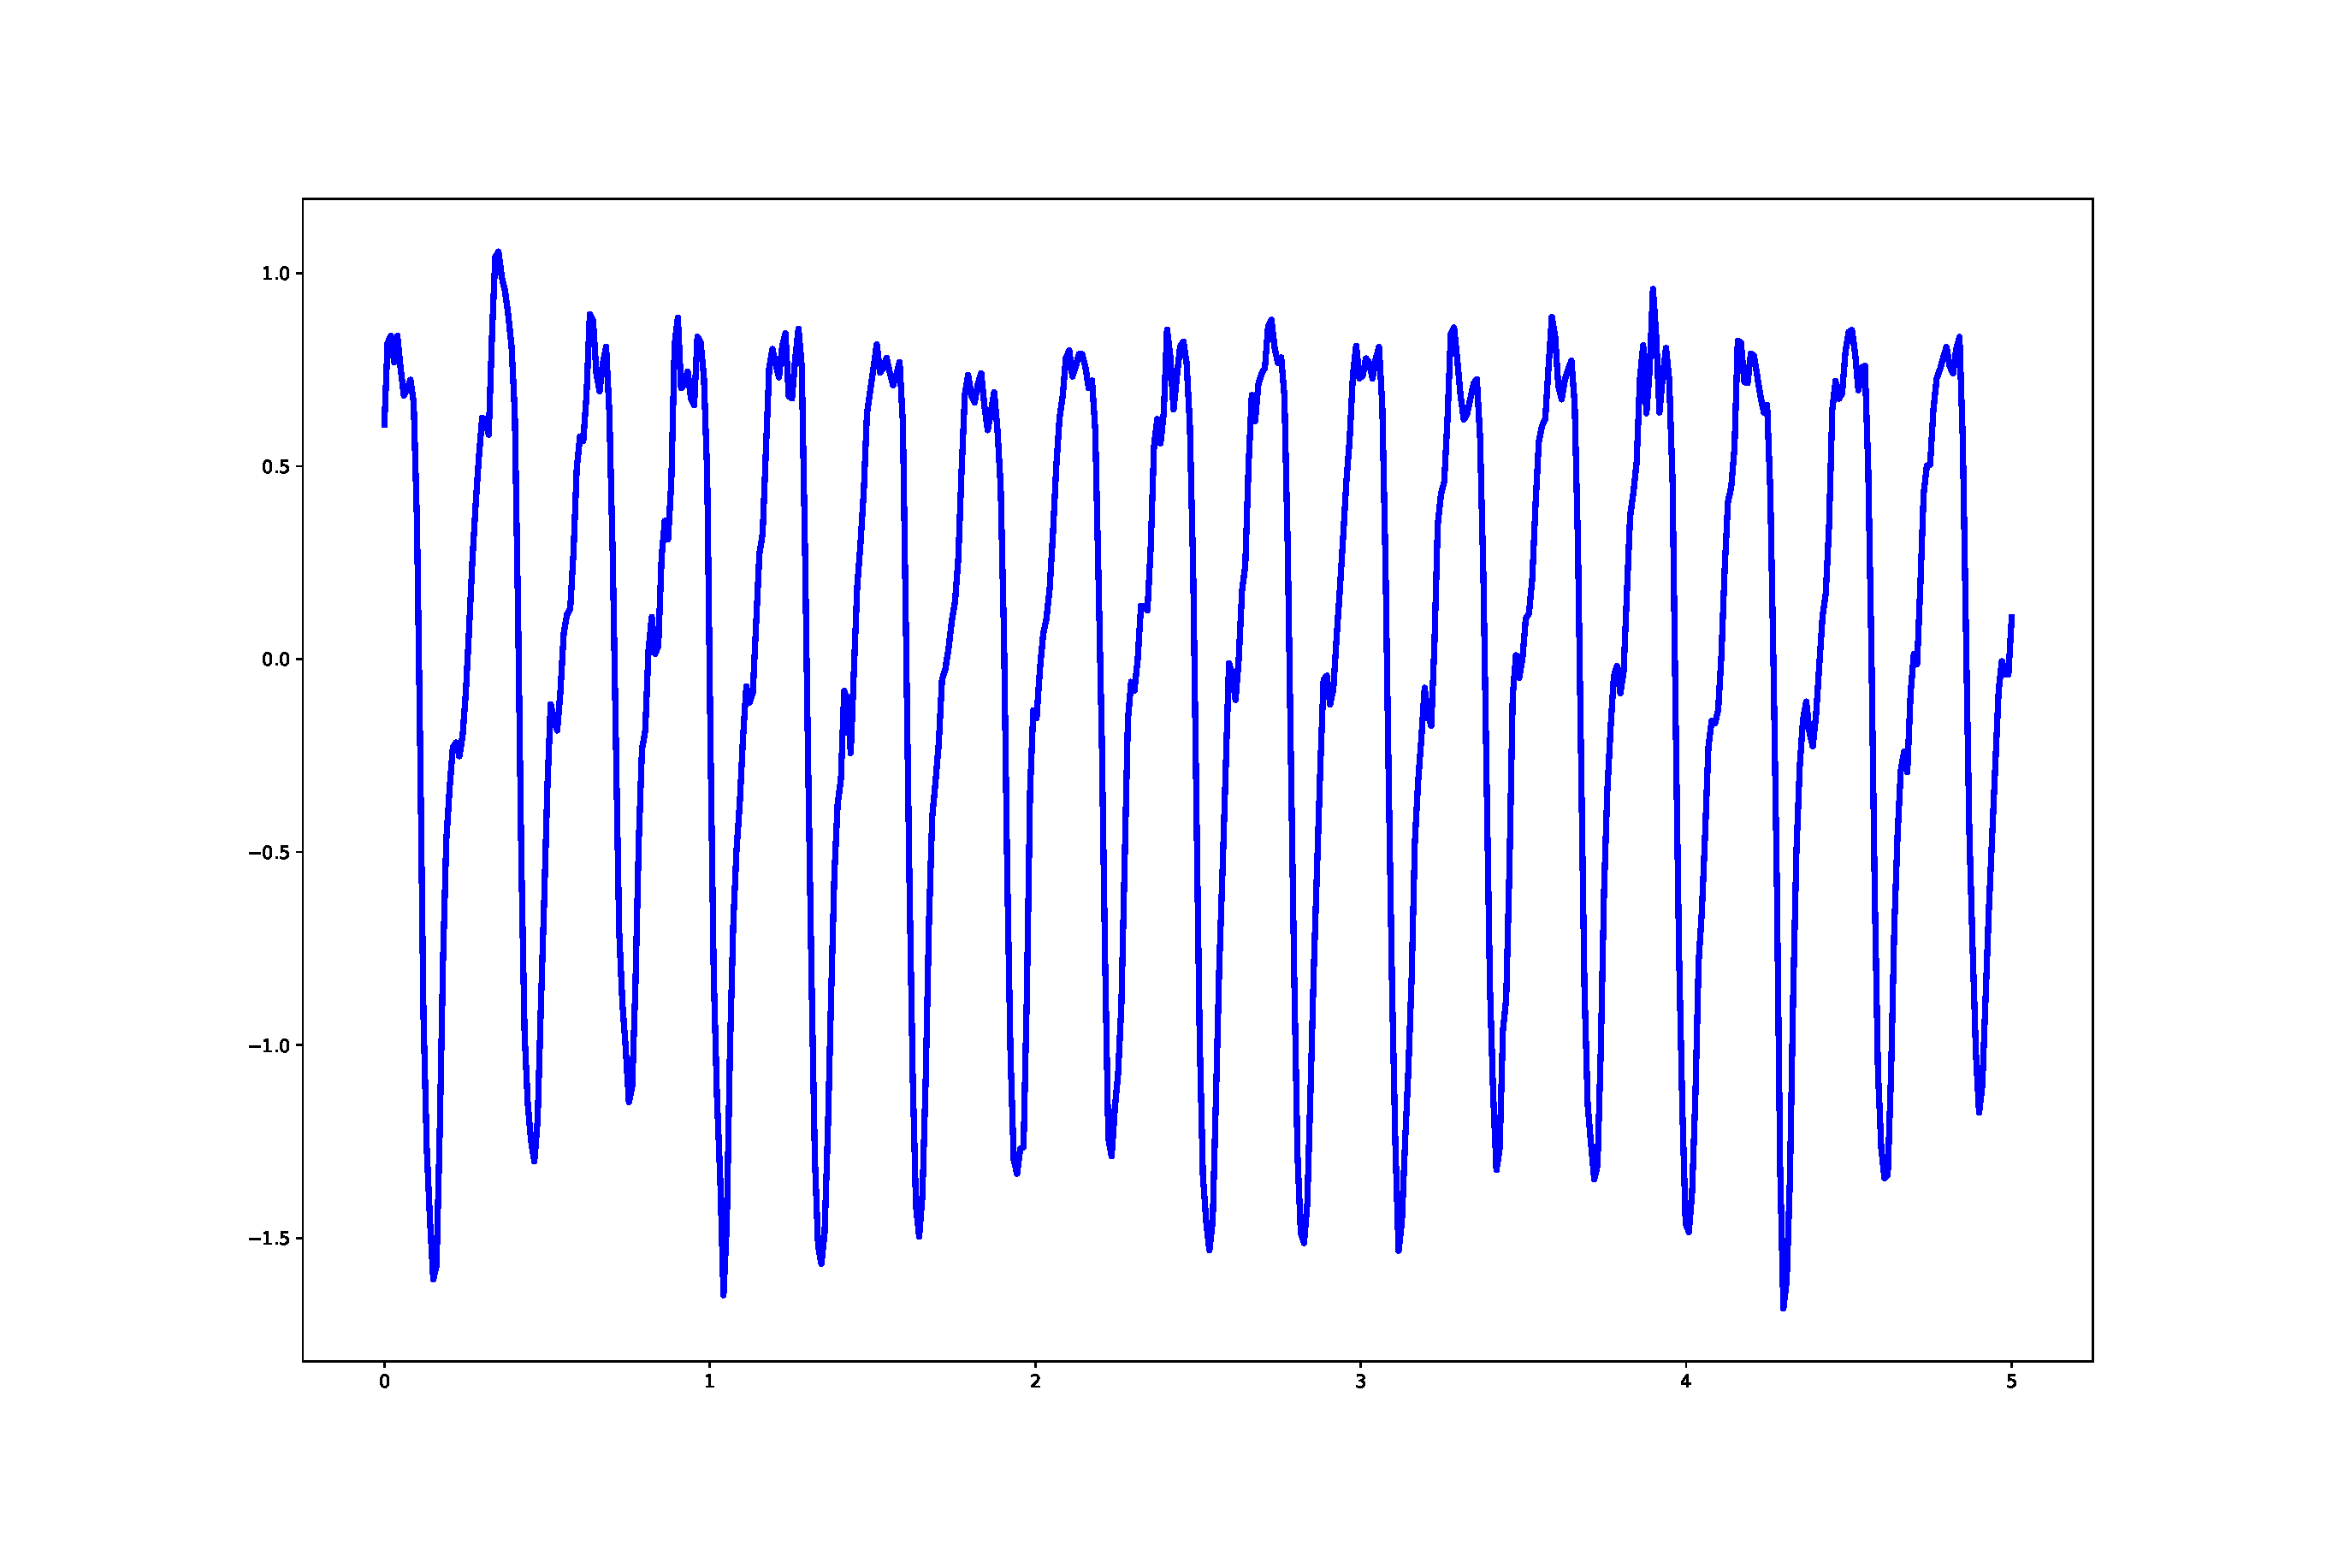
\includegraphics[width=1\linewidth]{images/ppg_example2}
			\caption{Example of a photoplethysmogram present in the database. The figure shows only the first part of the plot, that is much larger.}
			\label{fig:ppgexample}
		\end{figure}
		
		
		\section{The database}
			The database contains data coming from about 3600 patients. A PPG is saved in two arrays of the same length: the first one contains the signal, and the second one the time at which each signal of the first array has been recorded.  Two other important features used in this project and contained in the database, are the patient's age and a score related to the PPG quality.
			
			The other features of the database have not been used.
			\subsection{Preprocessing}
				The signals of the PPGs may not be always perfect: there could be some \emph{strange} peaks, or a very different behavior respect to the one in figure \ref{fig:ppgexample}.  This could be due to different factors, such as the pressure the patient push the finger with on the camera, or the position of the finger on the camera\dots These not \emph{well-behaving} PPGs must be removed from the database and, for this operation, the quality index is used. In this database lower the quality index is, the better the PPG is. For this reason I  set the a quality threshold at \colorbox{red}{0.005}, over the which the data are removed from the database. Doing this led to a number of usable PPGs to 3256. 
				A plate PPG has been removed manually because the quality threshold was not sufficeint to discriminate this particular PPG.
				
				\colorbox{red}{come sono presentati i dati}
		\section{Convolutional Variational Auto-Encoders}
			\label{vae_intro}
			\emph{Convolutional Variational Auto-Encorders} (CVAE) is an architecture of \emph{Deep Neural Network} (DNN). It can be used with different purposes, but in this project it has been used to perform an  \emph{unsupervised clustering}. This means that from the data we would like to divide them in clusters depending on the age of the patients, without providing the corresponding labels during the training phase of the Neural Network. 
			We can represent a CVAE using the scheme in Figure \ref{fig:vaebasic}. The data are provided to the input layer in the form of tensor, with a shape eqaul to (number of inputs, input height, input width, number of channel). That pass them to the \emph{encoder} that perform several convolution operations depending on the dimension of the input data. A convolutional layer can be described as a 
			\begin{figure}[h!] 
				\centering
				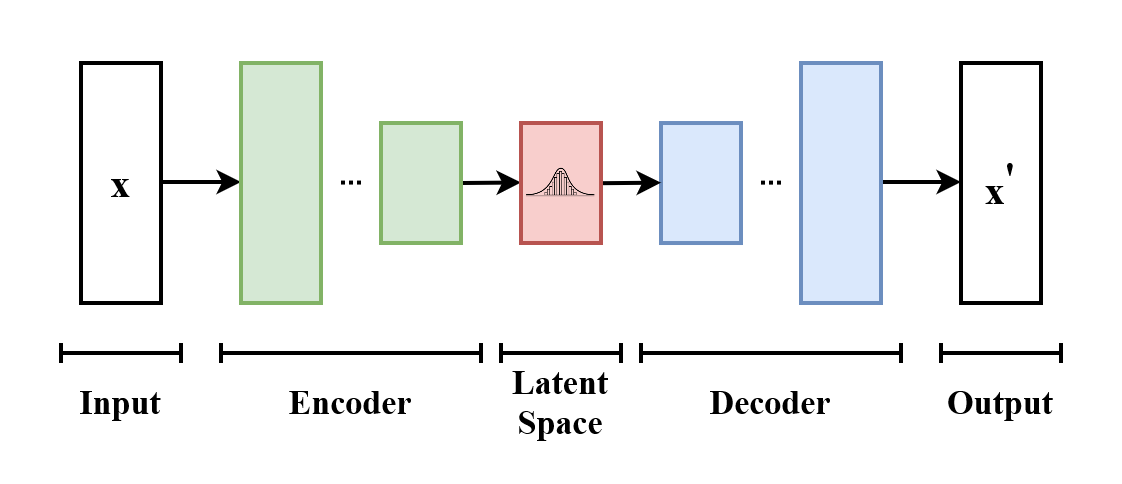
\includegraphics[width=1\linewidth]{images/VAE_Basic}
				\caption{In the structure of a CVAE, it is possible to distinguish the \emph{encoder}, that is composed by a Convolutional Network, the \emph{ latent space}, and the \emph{decoder}, that provide us the Neural Network output.}
				\label{fig:vaebasic}
			\end{figure}
		\newpage
		
		\printbibliography
\end{document}